\documentclass[colorlinks,empty,plainparagraph]{goose-article}

\newgeometry{left=25mm, right=25mm, top=30mm, bottom=22mm}
\setlength{\textfloatsep}{0.3em}

\title{Stress overshoot and fluidisation of a glass}
\author{Tom de Geus}
\hypersetup{pdfauthor={T.W.J. de Geus}}

\begin{document}

\twocolumn[
    \begin{@twocolumnfalse}
        \maketitle
    \end{@twocolumnfalse}
]
\sloppy

\paragraph*{Impact.}

How amorphous solids such as granular materials, bulk metallic glasses, colloidal suspensions or foams yield under an applied strain or flow under an applied stress is a central question in fields as diverse as geophysics, material science and soft matter.
This question enters your everyday life for example by the stability and manipulability of coffee foam, toothpaste, or mayonnaise.

\paragraph*{Background.}

Amorphous solids do not have a periodic structure of constituents but can respond elastically to an applied stress on experimental time scales.
The absence of a periodic structure can be achieved either by cooling a fluid too fast for the atoms to arrange themselves in a periodic structure, or by using a mixture of elements making the formation of a crystal sufficiently unlikely.
Regardless, without a periodic structure there are `no' defects either.
Yet the absence of order (i.e.\ the high-energy state of the arrangement of atoms) does mean that local rearrangements can occur.
Such rearrangements are not \emph{moving} defects as in the crystal, but they do introduce a restoring stress around the rearranging region, which can trigger rearrangements in neighbouring regions.
Curiously, once a rearrangement occurs, the region is again elastic (with a different elastic modulus and failure threshold).

\paragraph*{Model.}

It is common to study the response using a mesoscopic model that goes by the name of elastoplastic model.
In this model, the system is divided into a grid of elastically interacting `blocks', that are elastic and fail at a certain threshold.

\paragraph*{Shear banding.}

By arbitrarily choosing the initial distribution of failure thresholds larger than in the steady state, such that there is an initial slip weakening for each block, we have been able to show that a sheared glass, depending on the initial stability, can (1) yield smoothly, (2) smoothly overshoot, or (3) overshoot followed by catastrophic failure along a thin shear band.
\emph{Assuming} the existence of avalanches also in a stable glass (3), we argued that they form ``scars'' such that overall stability is governed by fracture mechanics.

\begin{figure}[htp]
    \centering
    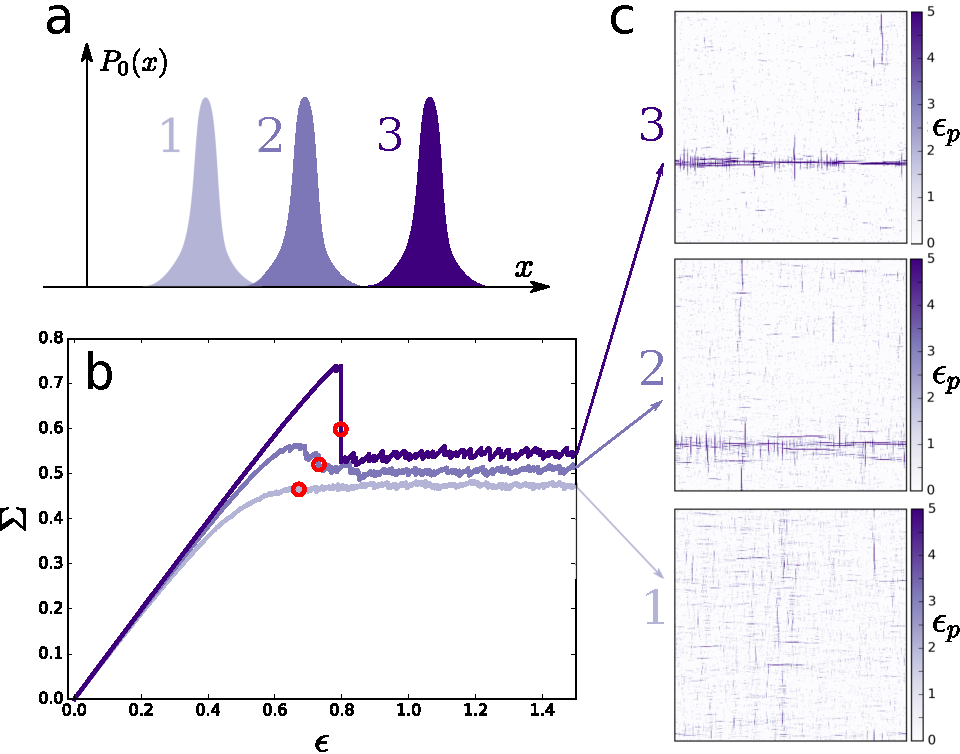
\includegraphics[width=\linewidth]{FigureSpatialResults.pdf}
\end{figure}

\paragraph*{Creep.}

When instead a stress is suddenly imposed, an amorphous solids display a transient creep flow.
The associated strain rate is commonly found to decay in time as $\dot{\gamma} \sim t^{-\nu}$, followed either by arrest or by a sudden fluidisation.
Various empirical laws have been suggested for the creep exponent $\nu$ and fluidisation time $\tau_f$.
We postulate that plastic flow is governed by the difference between the stress and a `transient yield stress', which is the maximal stress $\Sigma_t$ that the configurations visited at time $t$ can sustain without flowing.
Assuming the analyticity of $\Sigma_t$ allows us to predict $\nu$ and asymptotic behaviours of $\tau_f$ in terms of properties of stationary flows.

\begin{figure}[htp]
    \centering
    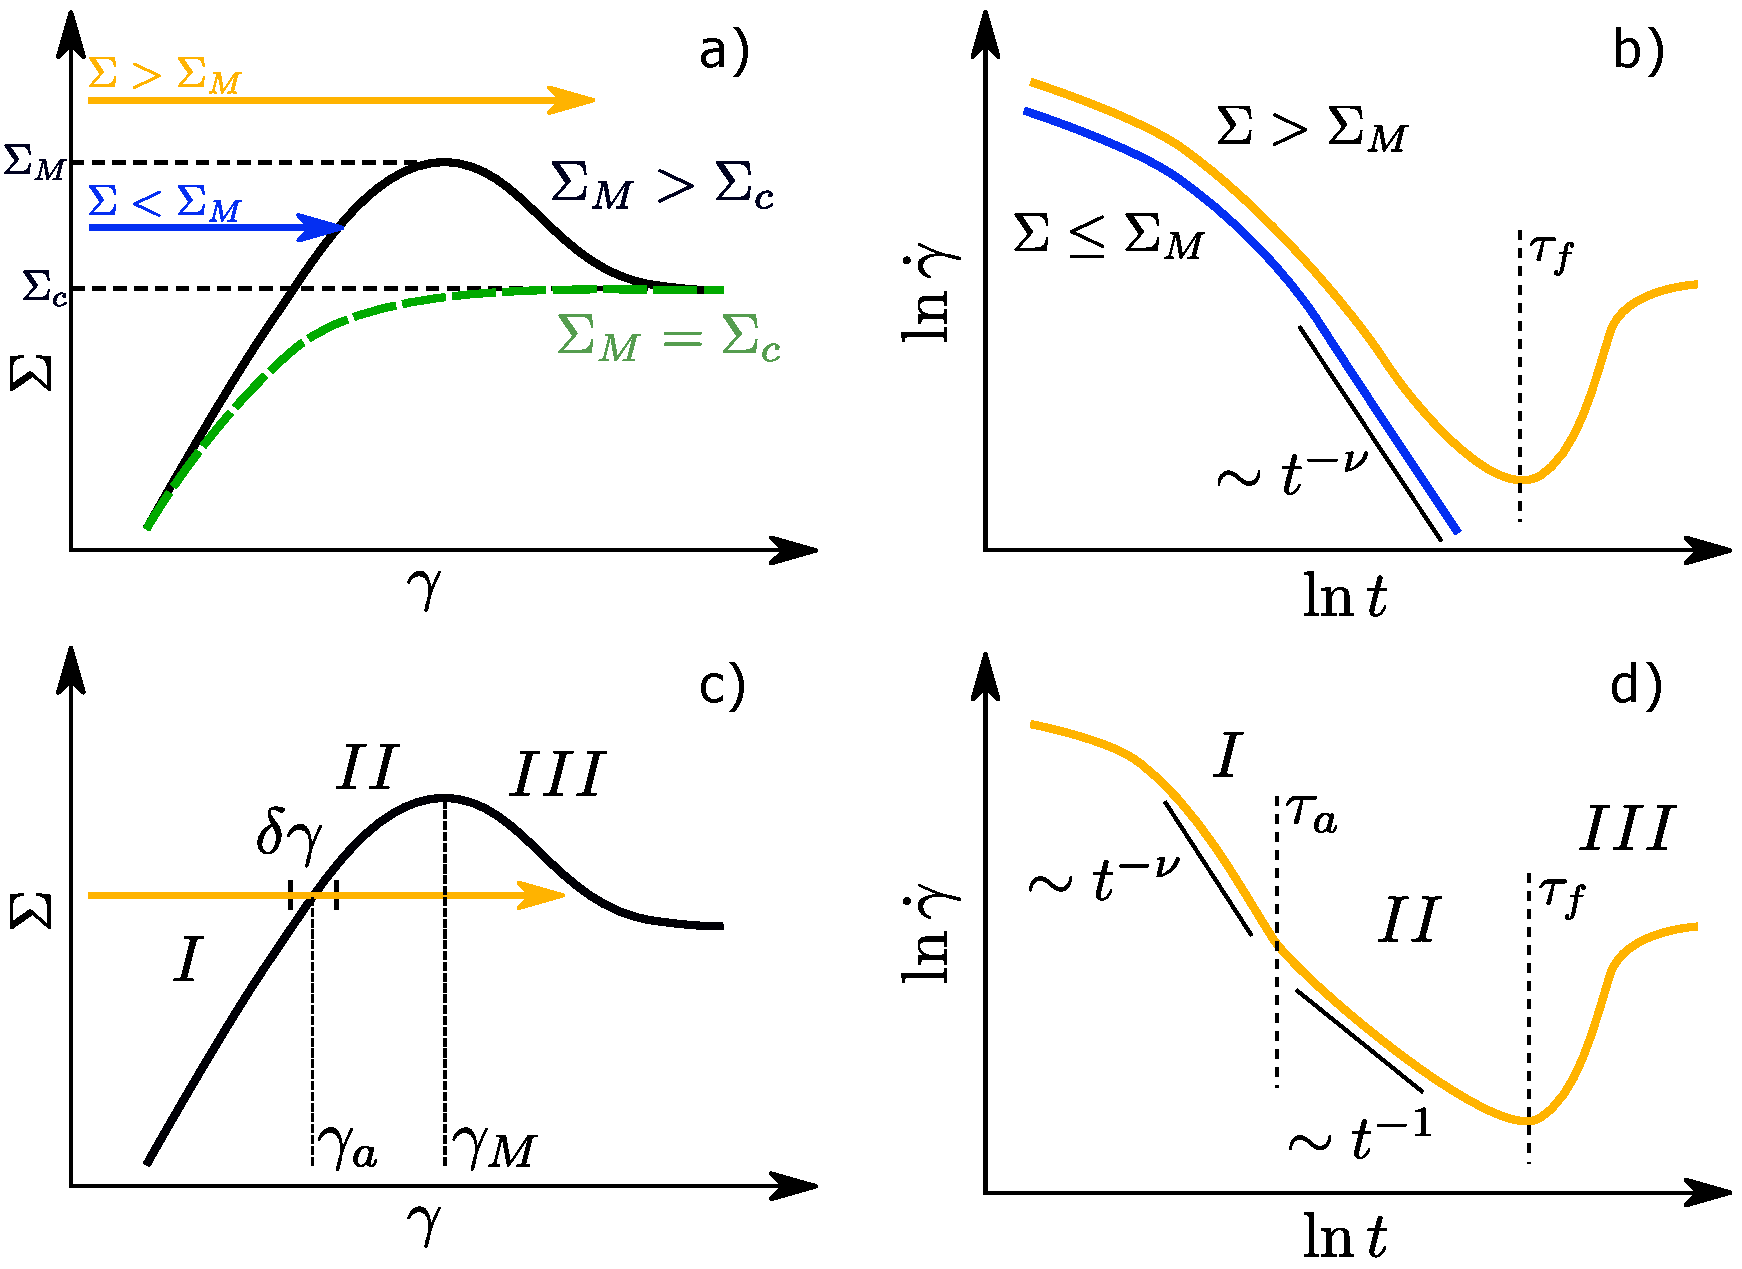
\includegraphics[width=\linewidth]{Figure1_TG.pdf}
\end{figure}

\nocite{Popovic2018,Popovic2021a}
\bibliographystyle{unsrtnat}
\renewcommand{\refname}{Selection of publications}
\bibliography{library}

\end{document}
